% Options for packages loaded elsewhere
\PassOptionsToPackage{unicode}{hyperref}
\PassOptionsToPackage{hyphens}{url}
\PassOptionsToPackage{dvipsnames,svgnames,x11names}{xcolor}
%
\documentclass[
  letterpaper,
  DIV=11,
  numbers=noendperiod]{scrartcl}

\usepackage{amsmath,amssymb}
\usepackage{iftex}
\ifPDFTeX
  \usepackage[T1]{fontenc}
  \usepackage[utf8]{inputenc}
  \usepackage{textcomp} % provide euro and other symbols
\else % if luatex or xetex
  \usepackage{unicode-math}
  \defaultfontfeatures{Scale=MatchLowercase}
  \defaultfontfeatures[\rmfamily]{Ligatures=TeX,Scale=1}
\fi
\usepackage{lmodern}
\ifPDFTeX\else  
    % xetex/luatex font selection
\fi
% Use upquote if available, for straight quotes in verbatim environments
\IfFileExists{upquote.sty}{\usepackage{upquote}}{}
\IfFileExists{microtype.sty}{% use microtype if available
  \usepackage[]{microtype}
  \UseMicrotypeSet[protrusion]{basicmath} % disable protrusion for tt fonts
}{}
\makeatletter
\@ifundefined{KOMAClassName}{% if non-KOMA class
  \IfFileExists{parskip.sty}{%
    \usepackage{parskip}
  }{% else
    \setlength{\parindent}{0pt}
    \setlength{\parskip}{6pt plus 2pt minus 1pt}}
}{% if KOMA class
  \KOMAoptions{parskip=half}}
\makeatother
\usepackage{xcolor}
\setlength{\emergencystretch}{3em} % prevent overfull lines
\setcounter{secnumdepth}{-\maxdimen} % remove section numbering
% Make \paragraph and \subparagraph free-standing
\ifx\paragraph\undefined\else
  \let\oldparagraph\paragraph
  \renewcommand{\paragraph}[1]{\oldparagraph{#1}\mbox{}}
\fi
\ifx\subparagraph\undefined\else
  \let\oldsubparagraph\subparagraph
  \renewcommand{\subparagraph}[1]{\oldsubparagraph{#1}\mbox{}}
\fi


\providecommand{\tightlist}{%
  \setlength{\itemsep}{0pt}\setlength{\parskip}{0pt}}\usepackage{longtable,booktabs,array}
\usepackage{calc} % for calculating minipage widths
% Correct order of tables after \paragraph or \subparagraph
\usepackage{etoolbox}
\makeatletter
\patchcmd\longtable{\par}{\if@noskipsec\mbox{}\fi\par}{}{}
\makeatother
% Allow footnotes in longtable head/foot
\IfFileExists{footnotehyper.sty}{\usepackage{footnotehyper}}{\usepackage{footnote}}
\makesavenoteenv{longtable}
\usepackage{graphicx}
\makeatletter
\def\maxwidth{\ifdim\Gin@nat@width>\linewidth\linewidth\else\Gin@nat@width\fi}
\def\maxheight{\ifdim\Gin@nat@height>\textheight\textheight\else\Gin@nat@height\fi}
\makeatother
% Scale images if necessary, so that they will not overflow the page
% margins by default, and it is still possible to overwrite the defaults
% using explicit options in \includegraphics[width, height, ...]{}
\setkeys{Gin}{width=\maxwidth,height=\maxheight,keepaspectratio}
% Set default figure placement to htbp
\makeatletter
\def\fps@figure{htbp}
\makeatother
\newlength{\cslhangindent}
\setlength{\cslhangindent}{1.5em}
\newlength{\csllabelwidth}
\setlength{\csllabelwidth}{3em}
\newlength{\cslentryspacingunit} % times entry-spacing
\setlength{\cslentryspacingunit}{\parskip}
\newenvironment{CSLReferences}[2] % #1 hanging-ident, #2 entry spacing
 {% don't indent paragraphs
  \setlength{\parindent}{0pt}
  % turn on hanging indent if param 1 is 1
  \ifodd #1
  \let\oldpar\par
  \def\par{\hangindent=\cslhangindent\oldpar}
  \fi
  % set entry spacing
  \setlength{\parskip}{#2\cslentryspacingunit}
 }%
 {}
\usepackage{calc}
\newcommand{\CSLBlock}[1]{#1\hfill\break}
\newcommand{\CSLLeftMargin}[1]{\parbox[t]{\csllabelwidth}{#1}}
\newcommand{\CSLRightInline}[1]{\parbox[t]{\linewidth - \csllabelwidth}{#1}\break}
\newcommand{\CSLIndent}[1]{\hspace{\cslhangindent}#1}

\usepackage{booktabs}
\usepackage{longtable}
\usepackage{array}
\usepackage{multirow}
\usepackage{wrapfig}
\usepackage{float}
\usepackage{colortbl}
\usepackage{pdflscape}
\usepackage{tabu}
\usepackage{threeparttable}
\usepackage{threeparttablex}
\usepackage[normalem]{ulem}
\usepackage{makecell}
\usepackage{xcolor}
\usepackage{amsmath}
\usepackage{caption}
%line numbers
%\usepackage{mathpazo}
%\usepackage{rotating}
\usepackage{lineno}
\linenumbers

\usepackage{rotfloat}
\KOMAoption{captions}{tableheading}
\makeatletter
\makeatother
\makeatletter
\makeatother
\makeatletter
\@ifpackageloaded{caption}{}{\usepackage{caption}}
\AtBeginDocument{%
\ifdefined\contentsname
  \renewcommand*\contentsname{Table of contents}
\else
  \newcommand\contentsname{Table of contents}
\fi
\ifdefined\listfigurename
  \renewcommand*\listfigurename{List of Figures}
\else
  \newcommand\listfigurename{List of Figures}
\fi
\ifdefined\listtablename
  \renewcommand*\listtablename{List of Tables}
\else
  \newcommand\listtablename{List of Tables}
\fi
\ifdefined\figurename
  \renewcommand*\figurename{Figure}
\else
  \newcommand\figurename{Figure}
\fi
\ifdefined\tablename
  \renewcommand*\tablename{Table}
\else
  \newcommand\tablename{Table}
\fi
}
\@ifpackageloaded{float}{}{\usepackage{float}}
\floatstyle{ruled}
\@ifundefined{c@chapter}{\newfloat{codelisting}{h}{lop}}{\newfloat{codelisting}{h}{lop}[chapter]}
\floatname{codelisting}{Listing}
\newcommand*\listoflistings{\listof{codelisting}{List of Listings}}
\makeatother
\makeatletter
\@ifpackageloaded{caption}{}{\usepackage{caption}}
\@ifpackageloaded{subcaption}{}{\usepackage{subcaption}}
\makeatother
\makeatletter
\@ifpackageloaded{tcolorbox}{}{\usepackage[skins,breakable]{tcolorbox}}
\makeatother
\makeatletter
\@ifundefined{shadecolor}{\definecolor{shadecolor}{rgb}{.97, .97, .97}}
\makeatother
\makeatletter
\makeatother
\makeatletter
\makeatother
\ifLuaTeX
  \usepackage{selnolig}  % disable illegal ligatures
\fi
\IfFileExists{bookmark.sty}{\usepackage{bookmark}}{\usepackage{hyperref}}
\IfFileExists{xurl.sty}{\usepackage{xurl}}{} % add URL line breaks if available
\urlstyle{same} % disable monospaced font for URLs
\hypersetup{
  pdftitle={Differences in COVID-19 vaccination in the province of Ontario across Health Regions and socio-economic strata},
  pdfauthor={Ariel Mundo Ortiz1,2; Bouchra Nasri1,2,},
  colorlinks=true,
  linkcolor={blue},
  filecolor={Maroon},
  citecolor={Blue},
  urlcolor={Blue},
  pdfcreator={LaTeX via pandoc}}

\title{\textbf{Differences in COVID-19 vaccination in the province of
Ontario across Health Regions and socio-economic strata}}
\author{}
\date{}

\begin{document}
\maketitle
\ifdefined\Shaded\renewenvironment{Shaded}{\begin{tcolorbox}[sharp corners, frame hidden, interior hidden, breakable, enhanced, borderline west={3pt}{0pt}{shadecolor}, boxrule=0pt]}{\end{tcolorbox}}\fi

\textsuperscript{1} Centre de Recherches Mathématiques, University of
Montreal, Montréal, Canada\\
\textsuperscript{2} Department of Social and Preventive Medicine, École
de Santé Publique, University of Montreal, Montréal, Canada

\textsuperscript{*} Correspondence:
\href{mailto:bouchra.nasri@umontreal.ca}{Bouchra Nasri
\textless{}bouchra.nasri@umontreal.ca\textgreater{}}

\hypertarget{abstract}{%
\section{Abstract}\label{abstract}}

The COVID-19 pandemic continues to be a worldwide public health concern.
Although vaccines against this disease were rapidly developed,
vaccination uptake has not ben equal across all the segments of the
population. In particular, it has been shown that there have been
differences in vaccine uptake across different segments of the
population. However, there are also differences in vaccination across
geographical areas, which might be important to consider in the
development of future public health policies against COVID-19. In this
study, we examined the relationship between vaccination status (having
received the first dose of a COVID-19 vaccine), and different
socio-economic and geographical factors. Our results show that during
the last three months of 2021, individuals in certain equity-deserving
groups (visible minorities) were three times less likely to be
vaccinated than White/Caucasian individuals across the province and that
in some cases, within these groups individuals in low income brackets
had significantly higher odds of vaccination when compared to their
peers in high income brackets. Finally, we identified significantly
lower odds of vaccination in the West Health Region of Ontario within
certain equity-deserving groups. This study shows that there is an
ongoing need to better understand and address differences in vaccination
uptake across diverse segments of the population of Ontario that have
been largely impacted by the pandemic.

\hypertarget{keywords}{%
\section*{Keywords}\label{keywords}}
\addcontentsline{toc}{section}{Keywords}

Covid-19, vaccination, survey, socio-economic factors, visible
minorities.

\hypertarget{background}{%
\section{Background}\label{background}}

The vaccines against COVID-19 have been considered a major achievement
of modern medicine as their rapid development allowed the start of broad
vaccination campaigns towards the end of 2020 in certain countries, such
as the US and
Canada\textsuperscript{\protect\hyperlink{ref-davis2022}{1}--\protect\hyperlink{ref-tanne2020}{3}}.
This made some believe that vaccines were destined to be a determinant
factor in a rapid ending of the
pandemic\textsuperscript{\protect\hyperlink{ref-thelancet2021}{4}}.
However, although it has been estimated that COVID-19 vaccines have
prevented around 14 million of deaths
worldwide\textsuperscript{\protect\hyperlink{ref-watson2022}{5}}, their
implementation has been far from being equal to that of the smallpox and
polio vaccines, which were implemented on a global scale and that were
crucial to control these
diseases\textsuperscript{\protect\hyperlink{ref-kayser2021}{6}}. In
fact, the rollout of COVID-19 vaccines has faced multiple challenges
since its inception which ultimately have hampered their use to achieve
the ultimate goal of global immunity.

This problematic in the rollout of the COVID-19 vaccines is a
multifaceted issue resulting from, among other things, the development
of new variants due to inadequate public health
measures\textsuperscript{\protect\hyperlink{ref-li2021}{7}}, inequality
in vaccine access between high- and low-income
countries\textsuperscript{\protect\hyperlink{ref-gerretsen2021}{8},\protect\hyperlink{ref-tamey2022}{9}},
vaccine
hesitancy\textsuperscript{\protect\hyperlink{ref-nafilyan2021}{10}}, and
differences in vaccination uptake across different segments of the
population\textsuperscript{\protect\hyperlink{ref-malik2020}{11}}. In
particular, it is well established that differences in vaccination
uptake have been present even in countries that have had ample access to
vaccines since 2020 (such as the US, the UK, and Canada), where lower
vaccine uptake has been observed within certain racial groups (i.e.,
individuals that identify as Black, Asian, or Indigenous), and in
individuals within low income
brackets\textsuperscript{\protect\hyperlink{ref-willis2021}{12}--\protect\hyperlink{ref-khubchandani2021}{15}}.
Reasons given for lower vaccine uptake in these cases have included
medical mistrust due to systemic medical
racism\textsuperscript{\protect\hyperlink{ref-stoler2021}{14}}, mistrust
in vaccines\textsuperscript{\protect\hyperlink{ref-willis2021}{12}}, and
the influence of conspiracy
theories\textsuperscript{\protect\hyperlink{ref-bogart2021}{16}--\protect\hyperlink{ref-freeman2020}{18}}.
Moreover, in the case of Canada, lower vaccine uptake has been observed
in young individuals, those with a low educational level, households
with children, those without a regular healthcare provider, individuals
that identify as part of certain equity-deserving groups, and those with
a low household
income\textsuperscript{\protect\hyperlink{ref-guay2022}{19}--\protect\hyperlink{ref-hussain2022}{21}}.

However, it is important to consider that vaccination uptake can also be
influenced by geographical (spatial) factors. In this regard,
differences in COVID-19 vaccination rates have been associated with
varied regional attitudes towards
vaccination\textsuperscript{\protect\hyperlink{ref-malik2020}{11}},
spatial differences in vaccine access and supply, vaccination location
availability, and lack of prioritization of areas where vulnerable
groups
reside\textsuperscript{\protect\hyperlink{ref-bogoch2022}{2},\protect\hyperlink{ref-nguyen2021}{22}}.
Other studies have also shown heterogeneity in vaccine uptake within
small governmental administrative units such as
counties\textsuperscript{\protect\hyperlink{ref-mollalo2021}{23}--\protect\hyperlink{ref-bhuiyan2022}{26}},
and that and that accounting for geographical differences in vaccination
can help predict patterns of booster
uptake\textsuperscript{\protect\hyperlink{ref-wood2022}{27}}. Overall,
the evidence provided by the literature demonstrates the existence of
spatially-driven heterogeneities in vaccine uptake that be used by
decision-makers in the development of public health policies that are
focused on addressing these disparities within specific administrative
or geographical areas.

However, such analyses have been carried mostly in territories outside
of Canada, where available studies have been focused in certain cities
(such as Toronto\textsuperscript{\protect\hyperlink{ref-choi2021}{28}},
or Montreal\textsuperscript{\protect\hyperlink{ref-mckinnon2021}{29}}),
or have explored differences at a province-wide
level\textsuperscript{\protect\hyperlink{ref-guay2022}{19}}. Thus, there
is a need for studies that explore spatial differences in vaccination
within the Canadian territory and that consequently, can help identify
disparities that need to be addressed within specific areas in each
province.

This need is particularly important in the case of Ontario, the most
populated province in Canada. Between 2006 and 2019, Ontario provided
healthcare access to its inhabitants using 14 intra-provincial divisions
called the Local Health Integrated Networks (LHINs). However, this
approach was complex, bureaucratic, and led to systemic
inequalities\textsuperscript{\protect\hyperlink{ref-tsasis2012}{30}}. In
late 2019, the 14 LHINs were phased out and the areas they covered were
incorporated into 6 Health Regions (North East, North West, Central,
Toronto, West, and East) in an effort to improve the healthcare system
of the province\textsuperscript{\protect\hyperlink{ref-dong2022}{31}}.
Because the adoption of the Health Regions is relatively recent, there
is an ongoing need to analyze the impact of this measure and identify
disparities in health access that might exist across the Health Regions,
which can be specially important in the context of the COVID-19
pandemic.

Therefore, in this study we hypothesized that there were differences in
vaccination uptake between the different Health Regions of Ontario
during the last quarter of 2021. By including socio-economic factors in
our analysis, we aimed at identifying in which groups these differences
were significant in order to provide an assessment of the current state
of healthcare access in Ontario.

\hypertarget{methods}{%
\section{Methods}\label{methods}}

\hypertarget{sec-data}{%
\subsection{Data and Methods}\label{sec-data}}

We used data from the \emph{Survey of COVID-19 related Behaviours and
Attitudes}, a repeated cross sectional survey focused on the Canadian
province of Ontario that was commissioned by the Fields Institute for
Research in Mathematical Sciences and the Mathematical Modelling of
COVID-19 Task Force under ethical guidance from the University of
Toronto, and which ran between September 30th, 2021 and January
17th,2022. The survey collected socio-economic information from
participants (Table~\ref{tbl-descriptive-stats}), their location
(nearest municipality, as shown in Figure~\ref{fig-map}), the date of
access to the survey, and asked information on vaccination status by
using the question ``Have you received the first dose of the COVID
vaccine?'', with possible answers ``yes'' and ``no''. The original
dataset contained 39,029 observations (where each observation
corresponded to a unique respondent).

Preliminary analyses of the data included the removal of outliers
(\textbf{should we still do this? it's only 19 observations with income
\textgreater110k and household of 1, but we are not even using such
income bracket in the analysis because we re-grouped the data, and the
household size variable has 90\% missing rate}), of observations where
respondents did not provide answers in all the covariates of interest,
matching the city of each observations with its corresponding LHIN and
Health Region, and removing observations from areas with low
representation (107 observations corresponding to the North West and
North East Health Regions). After all the preliminary analyses indicated
above, the total number of observations used for analysis was 3,549
which included the East, Central, Toronto, and West Health Regions
covering the period between October 1st,2021 and December 12th, 2021.
The original dataset, clean dataset, and details on the data cleaning
process are described in detail in the
\href{https://github.com/aimundo/Fields_COVID-19/}{GitHub repository}
for this paper.

\begin{figure}

{\centering 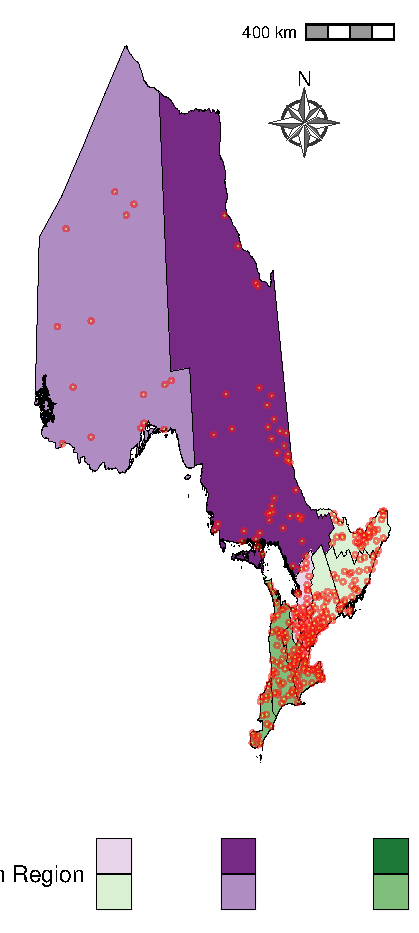
\includegraphics{../data/map_data/map.pdf}

}

\caption{\label{fig-map}Geographic representation of the data collected
by the \emph{Survey of COVID-19 related Behaviours and Attitudes},
collected by the Fields Institute in Ontario. The municipalities
(cities) from where survey participants provided answers (in the clean
dataset) appear as points. The Health six Regions are color-coded.
Internal boundaries within certain Health Regions indicate areas that
belonged to the Local Integrated Health Networks (LHINs), the geographic
areas for healthcare in Ontario before the adoption of the Health
Regions.}

\end{figure}

\hypertarget{statistical-analyses}{%
\subsection{Statistical analyses}\label{statistical-analyses}}

We used a logistic regression model to examine the impact of the Health
Regions in vaccination rates while considering the socio-economic
factors and and months covered by the survey
(Table~\ref{tbl-descriptive-stats}) and certain interactions (Race and
Health Region and Race and income), as previous studies have shown that
socio-economic factors and their interactions are significant predictors
of intent of vaccination and vaccination
status\textsuperscript{\protect\hyperlink{ref-nguyen2022}{32}--\protect\hyperlink{ref-cnat2022a}{34}}.
Because we identified differences in representativity between the survey
data and the estimates from the Census, we used an iterative
proportional fitting procedure
(\emph{raking})\textsuperscript{\protect\hyperlink{ref-deming1940}{35}}
to correct the data using data from the Census and Health Region
population totals; and fitted the regression model to the uncorrected
and corrected data. Details regarding the correction can be found in the
Appendix. All analyses were conducted in R 4.2.2 using the packages
\texttt{survey}\textsuperscript{\protect\hyperlink{ref-lumley2011}{36}},\texttt{tidyverse}\textsuperscript{\protect\hyperlink{ref-wickham2019}{37}},
\texttt{quarto}\textsuperscript{\protect\hyperlink{ref-quarto}{38}},
\texttt{modelsummary}\textsuperscript{\protect\hyperlink{ref-modelsummary}{39}},
and
\texttt{gtsummary}\textsuperscript{\protect\hyperlink{ref-gtsummary}{40}}.

\hypertarget{results}{%
\section{Results}\label{results}}

\hypertarget{sample-characteristics}{%
\subsection{Sample Characteristics}\label{sample-characteristics}}

Table~\ref{tbl-descriptive-stats} shows the characteristics of the data
from the Fields COVID-19 survey used for analysis. The sample contained
\textbf{6,236} observations, from which 24.8\% (1,547) corresponded to
individuals that reported not having received the first dose of the
vaccine. Vaccination rates ranged between 71-79\% across household
income brackets, age groups, Health Regions, and the months considered
in the survey. However, the highest vaccination rates in each category
were reported by individuals in the highest income bracket (79\%), those
between 16 and 34 years of age (77\%), individuals that lived in the
East Health Region (77\%), and during January of 2022 (78\%).
Differences were higher between racial/ethnic groups, where the higher
vaccination rate was reported by White/Caucasian individuals (84\%),
against vaccination rates between 63-66\% reported in the case of
Arab/Middle Eastern, Black, Indigenous, Latin American individuals, and
those that reported belonging to ``Other'' racial groups, which included
Southeast Asian, Filipino, West Asian, and minorities not identified
elsewhere.

\hypertarget{tbl-descriptive-stats}{}
\setlength{\LTpost}{0mm}
\begin{longtable}{lccc}
\caption{\label{tbl-descriptive-stats}Descriptive Statistics of the Fields COVID-19 Survey (by Vaccination
Status) }\tabularnewline

\toprule
\textbf{Variable} & \textbf{no}, N = 1,547\textsuperscript{1} & \textbf{yes}, N = 4,689\textsuperscript{1} & \textbf{p-value}\textsuperscript{2} \\ 
\midrule
Income (CAD) &  &  & <0.001 \\ 
    60000 and above & 542 (21\%) & 1,996 (79\%) &  \\ 
    25000-59999 & 347 (25\%) & 1,046 (75\%) &  \\ 
    under 25000 & 658 (29\%) & 1,647 (71\%) &  \\ 
Age Group &  &  & 0.002 \\ 
    16-34 & 645 (23\%) & 2,117 (77\%) &  \\ 
    35-54 & 411 (24\%) & 1,305 (76\%) &  \\ 
    55 and over & 491 (28\%) & 1,267 (72\%) &  \\ 
Health Region &  &  & 0.3 \\ 
    Toronto & 593 (26\%) & 1,709 (74\%) &  \\ 
    Central & 372 (26\%) & 1,083 (74\%) &  \\ 
    East & 236 (23\%) & 783 (77\%) &  \\ 
    West & 346 (24\%) & 1,114 (76\%) &  \\ 
Month &  &  & <0.001 \\ 
    October & 469 (27\%) & 1,263 (73\%) &  \\ 
    November & 376 (28\%) & 980 (72\%) &  \\ 
    December & 181 (24\%) & 565 (76\%) &  \\ 
    January & 521 (22\%) & 1,881 (78\%) &  \\ 
Race &  &  & <0.001 \\ 
    White/Caucasian & 354 (16\%) & 1,871 (84\%) &  \\ 
    Arab/Middle Eastern & 111 (34\%) & 220 (66\%) &  \\ 
    Black & 159 (34\%) & 303 (66\%) &  \\ 
    East Asian/Pacific Islander & 94 (19\%) & 404 (81\%) &  \\ 
    Indigenous & 112 (37\%) & 194 (63\%) &  \\ 
    Latin American & 99 (34\%) & 195 (66\%) &  \\ 
    Mixed & 177 (30\%) & 411 (70\%) &  \\ 
    Other\textsuperscript{3} & 315 (34\%) & 606 (66\%) &  \\ 
    South Asian & 126 (21\%) & 485 (79\%) &  \\ 
\bottomrule
\end{longtable}
\begin{minipage}{\linewidth}
\textsuperscript{1}n (\%)\\
\textsuperscript{2}Pearson\textquotesingle{}s Chi-squared test\\
\textsuperscript{3}Southeast Asian, Filipino, West Asian,
and minorities not identified elsewhere according to the Census.\\
\end{minipage}

\hypertarget{multivariate-regression}{%
\subsection{Multivariate Regression}\label{multivariate-regression}}

Figure~\ref{fig-model-uncorr} shows the estimates from the logistic
regression model of vaccination status for the uncorrected data, whereas
the estimated obtained from the corrected data appear in
Figure~\ref{fig-model-corr}. The results show significantly lower odds
of vaccination in individuals with a low household income and those that
identified as part of equity-deserving groups when compared to
individuals in high income brackets or that identified as White or
Caucasian.

\begin{figure}

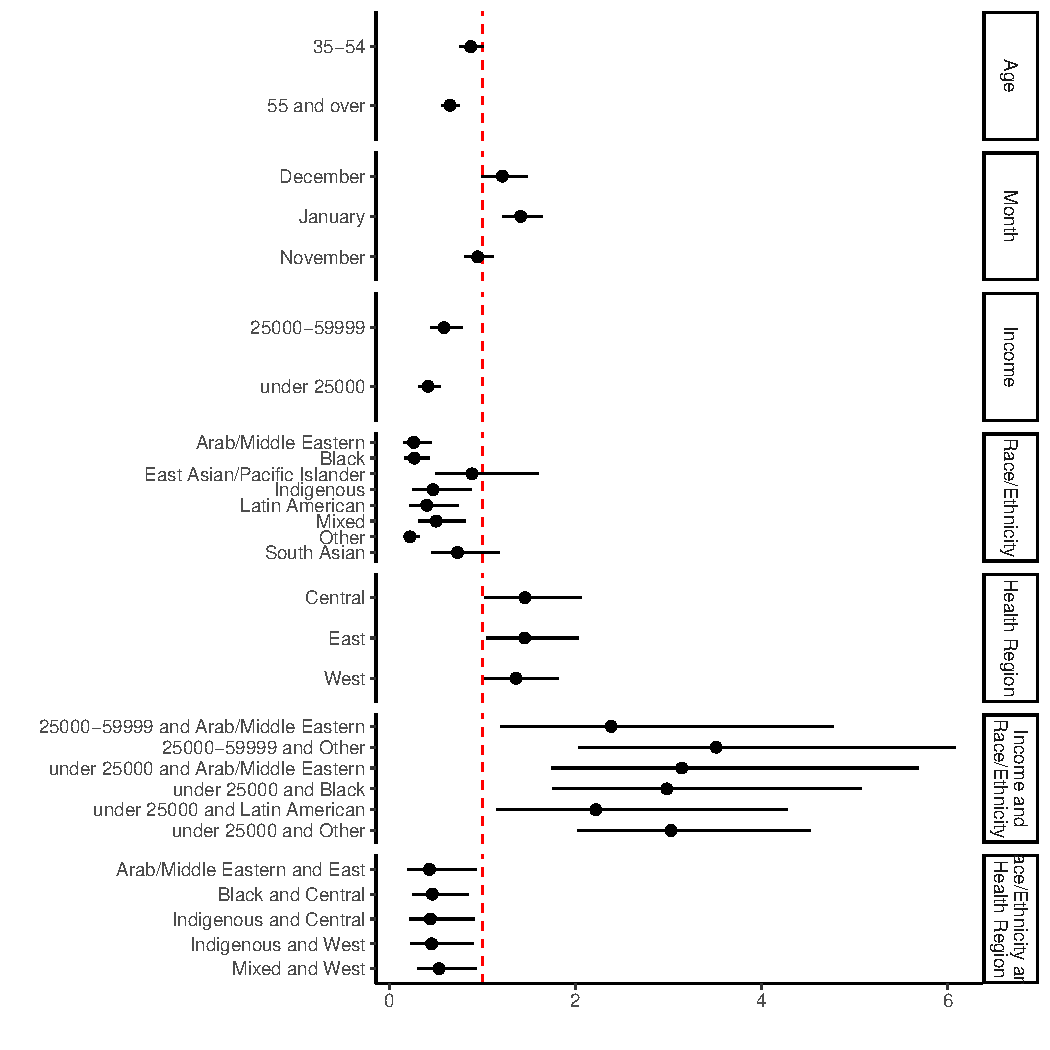
\includegraphics{main_files/figure-pdf/fig-model-uncorr-1.pdf} \hfill{}

\caption{\label{fig-model-uncorr}Coefficient estimates and confidence
intervals for the uncorrected model. Only statistically significant
interaction terms are shown. Full interaction terms can be found in
Supplementary Figure A-3.}

\end{figure}

Specifically, significantly lower odds of vaccination were identified
for those with a household income under CAD 25,000 (OR=0.37,
CI={[}0.25,0.56{]}) and those with an income between CAD 25,000 and
59,999 (OR=0.59, CI={[}0.39,0.88{]}). Additionally, individuals who
identified as Arab/Middle Eastern, Black, or Latin American, or that
belonged to ``Other'' racial groups, which included the Southeast Asian,
Filipino, West Asian, and Minorities Not Identified Elsewhere groups
according to the Census, had significantly lower odds of vaccination
than those in the White/Caucasian group (ORs=0.31, 0.32, 0.27, 0.22, and
CIs={[}0.14,0.68{]}, {[}0.17,0.60{]}, {[}0.11,0.66{]}, and
{[}0.12,0.41{]}, respectively). Regarding Health Regions, individuals
that reported living in the West Health Region (which includes the
regions of Waterloo and Niagara, the counties of Wellington, Essex, and
Lambton, and the cities of Hamilton, Haldimand, Brant, and Chatham-Kent)
had significantly higher odds of vaccination than those in the Health
Region of Toronto (OR=1.54, CI={[}1.04,2.29{]}).

Interestingly, individuals in equity-deserving groups with a household
income below CAD 25,000 had higher odds of vaccination (when compared to
those with a household income above CAD 60,000). This held true in the
case of Arab/Middle Eastern (OR=3.08, CI={[}1.27,7.47{]}), Black
(OR=3.15, CI={[}1.43,6.92{]}), and Latin American (OR=2.81,
CI={[}1.04,7.59{]}) individuals, as well as respondents who belonged to
``Other'' minority groups (OR=4.63, CI={[}2.34,9.13{]}), who also had
higher odds of vaccination in the CAD 25,000-59,999 income bracket
(OR=6.96, CI={[}2.67,18.16{]}). Finally, significantly lower odds of
vaccination were identified (when compared to the Toronto Health Region)
for Black individuals in the Central Health Region, which comprises the
region of York, counties of Dufferin and Simcoe and the district of
Muskoka (OR=0.44, CI={[}0.19,0.99{]}), and in individuals that
identified as part of other racial minorities or South Asian that lived
in the West Health Region (ORs=0.41, and CIs={[}0.18,0.92{]} and
{[}0.18,0.95{]}, respectively).

\begin{figure}

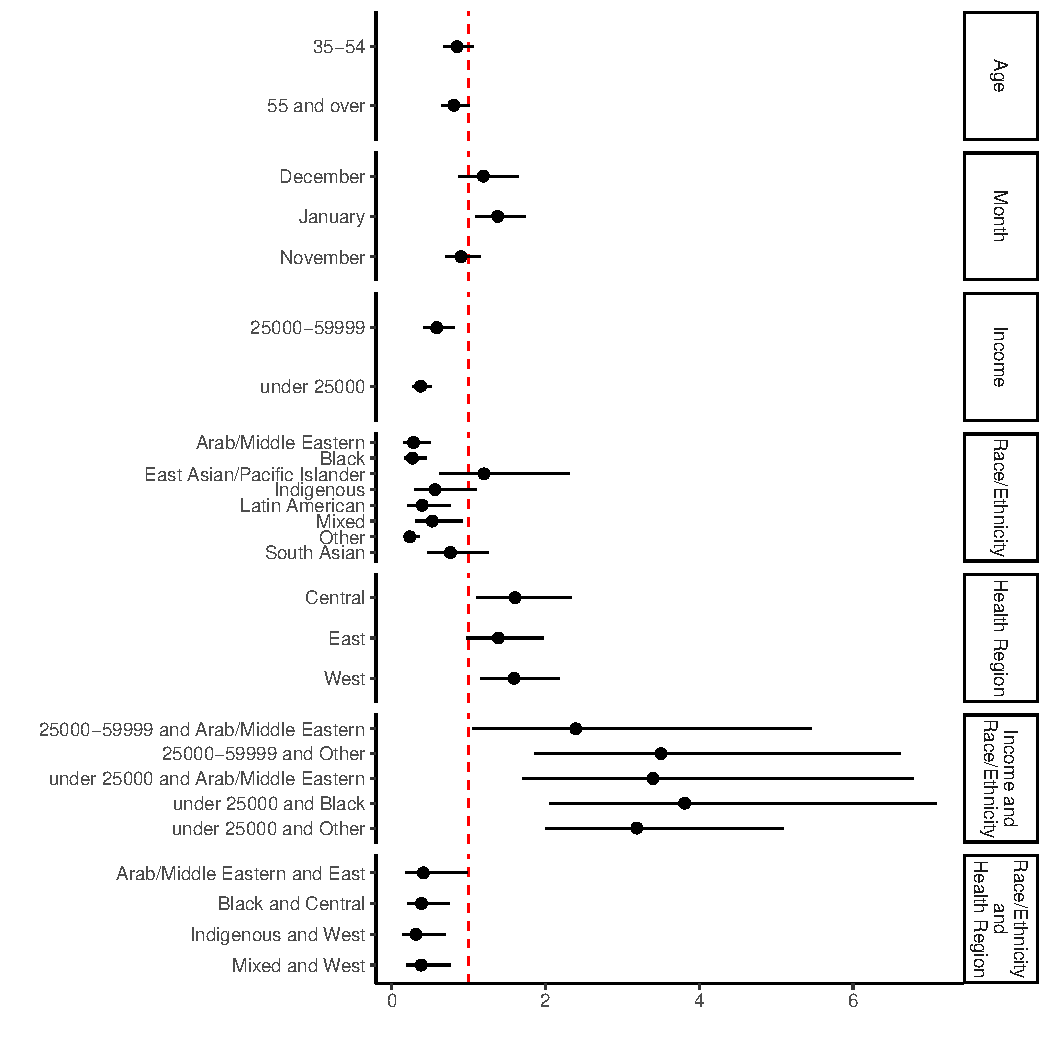
\includegraphics{main_files/figure-pdf/fig-model-corr-1.pdf} \hfill{}

\caption{\label{fig-model-corr}Coefficient estimates and confidence
intervals for the corrected model. Only statistically significant
interaction terms are shown. Full interaction terms can be found in
Supplementary Figure A-4.}

\end{figure}

\hypertarget{discussion}{%
\section{Discussion}\label{discussion}}

The existence of healthcare disparities in Ontario motivated the recent
change in the healthcare system of the province, which switched from the
LHIN model to the Health Region model in late
2019\textsuperscript{\protect\hyperlink{ref-tsasis2012}{30},\protect\hyperlink{ref-dong2022}{31}}.
This change is relatively recent, and because of this, is likely that
there are ongoing differences in healthcare access across the province.
In this study we hypothesized that differences in COVID-19 vaccination
uptake were present between the Health Regions, aiming at determining
which socio-demographic groups could be impacted by these disparities
and to provide decision-makers with information that could be used to
develop policies focused on reducing or eliminating these differences
and ensure that the Health Region model is able to improve health access
for the inhabitants of Ontario, a province that faces unique challenges
due to its condition as the most populated and the most ethnically
diverse province of Canada.

Our results indicate that across the most densely populated Health
Regions of Ontario, almost three quarters of surveyed individuals
reported to have received the first dose of the COVID-19 vaccine
(Table~\ref{tbl-descriptive-stats}). We identified significant
intra-provincial differences in vaccination based on socio-economic and
geographical factors. First, our results show differences in odds of
vaccination in individuals with a household income below CAD 60,000 and
in individuals belonging to visible minority groups. Those who
identified as Arab/Middle Eastern, Black, Latin American, or that
belonged to a minority group not included in the survey (Southeast
Asian, Filipino, West Asian, and minority groups not identified
elsewhere) had vaccination odds that were less than a third of
individuals that identified as White/Caucasian
(Figure~\ref{fig-model-corr}). These results are consistent with other
studies that have shown lower vaccination rates in individuals that
identify as part of a racial minority, or that have a low household
income\textsuperscript{\protect\hyperlink{ref-guay2022}{19}--\protect\hyperlink{ref-hussain2022}{21},\protect\hyperlink{ref-carter2022}{41}}.
In the case of Ontario, a possible rationale for this difference is
vaccine access, which has been identified as an important contributing
factor of disparities in vaccination for equity-deserving
groups\textsuperscript{\protect\hyperlink{ref-njoku2021}{42}}, and that
occurred in Toronto earlier in 2021, where it has been shown that
vaccination venues were scarce in low socio-economic areas that had the
highest burden of COVID-19 at the
time\textsuperscript{\protect\hyperlink{ref-bogoch2022}{2}}.

It is interesting to note that although overall self-reported
vaccination rates were found to be statistically significantly lower in
various racial minority groups when compared to White/Caucasian
individuals, the change in odds of vaccination within certain racial
groups and income strata was actually positive, in contrast to the
White/Caucasian group, where vaccination odds decreased in lower income
brackets (when compared to the CAD 60,000 and over bracket,
Supplementary Figure A-5). More specifically, the change in odds of
vaccination increased in individuals who identified as Arab/Middle
Eastern, Black, Latin American, or belonging to other minority groups
with a household income below CAD 25,000, which was also true for
individuals in other racial minority groups with an income between CAD
25,000-59,999.

This result is likely due in part to the fact that individuals that
belong racial minority groups tend to perform occupations that have been
deemed as ``essential'' in the context of the
pandemic\textsuperscript{\protect\hyperlink{ref-hawkins2020}{43},\protect\hyperlink{ref-ct2021}{44}},
which include grocery store workers, gas station, warehouse,
distribution, and manufacturing workers, all being occupations for which
an income within the significant brackets identified in the analysis is
to be expected. In the case of Ontario, essential workers had priority
for COVID-19
vaccination\textsuperscript{\protect\hyperlink{ref-mishra2021}{45}},
which would explain the higher odds of vaccination for these
individuals. In other words, it is possible that the type of occupation
from individuals in equity-deserving groups played an important role in
increasing the odds of vaccination.

Additionally, significant higher vaccination odds were identified in the
West Health Region when compared to the Health Region of Toronto
(Figure~\ref{fig-model-corr}). The West Health Region comprises the
regions of Waterloo and Niagara, the counties of Wellington, Essex and
Lambton, and the cities of Hamilton, Haldimand, Brant, and Chatham-Kent.
In this case, these results could reflect the fact that in the survey,
about half of the entries for this Health Region corresponded to
White/Caucasian individuals, who reported a vaccination rate of 83\%
(Supplementary Table A-6). However, the interaction effect of Health
Region and race was also significant in the case of individuals
identifying as South Asian or other minorities not included in the
survey Figure~\ref{fig-model-corr}. In this case, the results of the
interaction term in the model indicate that the odds of vaccination for
those within the South Asian and Other minority groups in the West
Region decreased when compared to the other Health Regions
(Supplementary Figure A-6).

According to Ontario Health, 13.2\% of the population in the West Health
Region identifies as a visible minority, whereas 2.5\% identifies as
Indigenous\textsuperscript{\protect\hyperlink{ref-ontariohealth}{46}}.
Therefore, the estimated lower odds are likely to be explained from a
socio-economic perspective. In fact, 50\% of the answers from this
region in the survey came from the former LHINs of Hamilton Niagara
Haldimand Brant, and Erie St.~Clair, both which are among the regions of
Ontario with the highest proportion of their population (more than 20\%)
in the lowest income
quintile\textsuperscript{\protect\hyperlink{ref-buajitti2018}{47}}
(Supplementary Table A-7). Interestingly, a disproportionate number of
COVID-19 cases and low vaccination rate (under 50\%) have been also
reported in the South Asian community of
Ontario\textsuperscript{\protect\hyperlink{ref-anand2022}{48}}. These
results provide context to the observed differences in vaccination among
the Health Regions of the province, showing which equity-deserving and
socio-demographic groups in certain regions need to be prioritized in
future vaccination strategies. Moreover, these results provide a
rationale for future studies that explore how vaccination uptake varies
across different minority groups within Ontario and other Canadian
provinces.

There are some limitations to the present study. First, the data
collection design, which allowed respondents to withdraw from the survey
at any point, resulted in a high number of unique entries in the survey
with multiple missing answers. Because we focused on entries that had
complete observations in the covariates of interest for our analysis, it
is possible that some information was not considered by excluding
observations that had information in other variables (such as work from
home, or number of persons in the household). However, we attempted to
minimize this possibility by correcting the dataset using information
from the Census. More granular corrections, which for example could be
based on demographic information by municipality, could be used in the
future to obtain a more accurate approximation to the population totals
of the province. Moreover, our analysis did not consider the North West
and North East Health Regions, due to the low number of entries from
these areas in the survey (Figure~\ref{fig-map}). Although low
representation from these areas is based on the fact that these regions
only account for 5\% of the total population of Ontario, these regions
are the home to more than 100,000 individuals that identify as
Indigenous\textsuperscript{\protect\hyperlink{ref-ontariohealth}{46}}, a
minority group that has historically suffered from reduced access to
health care and
discrimination\textsuperscript{\protect\hyperlink{ref-mosby2021}{17}}.
Therefore, there is a need for additional studies that focus on these
low-populated Health Regions in Ontario where disparities in vaccination
might be significant and understudied.

It is also worth mentioning that province-wide vaccination rates for the
period of interest are somewhat different from those of the survey,
particularly in the case of those 55 years of age and older, which in
the survey had a vaccination rate of 72\%, against a rate of 88.4\%
reported for the closest age bracket (50 years of age and older)
reported by Public Health Ontario at the start of the period covered by
the data\textsuperscript{\protect\hyperlink{ref-ontario-covid}{49}}.
However, we found good agreement between the estimates from the model
and overall vaccination rates reported for Canada, which have been
relatively higher when compared to other high income
countries\textsuperscript{\protect\hyperlink{ref-dube2022}{50}}, and
with vaccination uptake rates across different age groups presented in
other
studies\textsuperscript{\protect\hyperlink{ref-guay2022}{19},\protect\hyperlink{ref-macdonald2021}{51}}.

In other words, although vaccination rates obtained from the survey were
slightly lower than the provincial estimates, these values still
represented a valid approximation to overall trends; this notion is
reinforced by the consistency in the proportion of vaccination rates
(Table~\ref{tbl-descriptive-stats}) and vaccination odds
(Figure~\ref{fig-model-corr}) across the period covered by the survey,
which closely match the vaccination rates from Public Health Ontario and
which indicate that due to the relatively high coverage achieved in the
population at that point, vaccination rates increased by around 3\%
across all age groups during the three months covered by the
survey\textsuperscript{\protect\hyperlink{ref-ontario-covid}{49}}. It is
also important to mention that to this day, differences in vaccination
rates within the province continue. As of March of 2023 some regions
still have less than 75\% vaccination
rate\textsuperscript{\protect\hyperlink{ref-ontario-covid-map}{52}}, and
although data for the period analyzed in this study is not
publicly-available, it is likely that differences in vaccination rates
were higher at the time, being partially captured by the survey.

The results in this study are based on self-reported data, where bias
might be present. However, because in the context of COVID-19 it has
been shown that good agreement exists between self-reported and
documented vaccination
status\textsuperscript{\protect\hyperlink{ref-stephenson2022}{53}}, we
believe that our data was able to provide a valid assessment of
vaccination in the province. Finally, this study focused on first-dose
vaccination status within a relatively short time window, and therefore
can only provide a snapshot of the societal dynamics behind the
pandemic. Nonetheless, the results presented here can serve as a
starting point to motivate the collection of robust longitudinal data
that can be used to quantify geographical and temporal differences
within vulnerable segments of the population, and that can be used to
inform the development of adequate public health policies within the
province of Ontario or across other provinces that aim to minimize
disparities in health access.

\hypertarget{conclusion}{%
\section{Conclusion}\label{conclusion}}

This study explored differences in COVID-19 vaccination across the
province of Ontario during the last quarter of 2021 taking into
consideration socio-economic factors, such as income and race, their
interactions, and the Health Regions within the province. Our results
show that during the period analyzed, differences in vaccination uptake
existed across multiple equity-deserving groups in the province, and
that these differences were significant in two of the Health Regions
analyzed. It is important that future public health policies in Ontario
take into consideration how to adequately reach individuals from
equity-deserving groups that might live in areas of the province where
access to healthcare might be difficult. Only in this way the goal of
the Health Region model, which aims at reducing disparities, will become
successful.

\hypertarget{references}{%
\section{References}\label{references}}

\hypertarget{refs}{}
\begin{CSLReferences}{0}{0}
\leavevmode\vadjust pre{\hypertarget{ref-davis2022}{}}%
\CSLLeftMargin{1. }%
\CSLRightInline{Davis CJ, Golding M, McKay R. Efficacy information
influences intention to take COVID-19 vaccine. \emph{British Journal of
Health Psychology}. 2022;27(2):300-319.
doi:\url{https://doi.org/10.1111/bjhp.12546}}

\leavevmode\vadjust pre{\hypertarget{ref-bogoch2022}{}}%
\CSLLeftMargin{2. }%
\CSLRightInline{Bogoch II, Halani S. {COVID}-19 vaccines: A geographic,
social and policy view of vaccination efforts in ontario, canada.
\emph{Cambridge Journal of Regions, Economy and Society}. Published
online November 2022.
doi:\href{https://doi.org/10.1093/cjres/rsac043}{10.1093/cjres/rsac043}}

\leavevmode\vadjust pre{\hypertarget{ref-tanne2020}{}}%
\CSLLeftMargin{3. }%
\CSLRightInline{Tanne JH. Covid-19: {FDA} panel votes to authorise
pfizer {BioNTech} vaccine. \emph{{BMJ}}. Published online December
2020:m4799.
doi:\href{https://doi.org/10.1136/bmj.m4799}{10.1136/bmj.m4799}}

\leavevmode\vadjust pre{\hypertarget{ref-thelancet2021}{}}%
\CSLLeftMargin{4. }%
\CSLRightInline{Microbe TL. {COVID}-19 vaccines: The pandemic will not
end overnight. \emph{The Lancet Microbe}. 2021;2(1):e1.
doi:\href{https://doi.org/10.1016/s2666-5247(20)30226-3}{10.1016/s2666-5247(20)30226-3}}

\leavevmode\vadjust pre{\hypertarget{ref-watson2022}{}}%
\CSLLeftMargin{5. }%
\CSLRightInline{Watson OJ, Barnsley G, Toor J, Hogan AB, Winskill P,
Ghani AC. Global impact of the first year of {COVID}-19 vaccination: A
mathematical modelling study. \emph{The Lancet Infectious Diseases}.
2022;22(9):1293-1302.
doi:\href{https://doi.org/10.1016/s1473-3099(22)00320-6}{10.1016/s1473-3099(22)00320-6}}

\leavevmode\vadjust pre{\hypertarget{ref-kayser2021}{}}%
\CSLLeftMargin{6. }%
\CSLRightInline{Kayser V, Ramzan I. Vaccines and vaccination: History
and emerging issues. \emph{Human Vaccines {\&}amp\(\mathsemicolon\)
Immunotherapeutics}. 2021;17(12):5255-5268.
doi:\href{https://doi.org/10.1080/21645515.2021.1977057}{10.1080/21645515.2021.1977057}}

\leavevmode\vadjust pre{\hypertarget{ref-li2021}{}}%
\CSLLeftMargin{7. }%
\CSLRightInline{Li Q, Wang J, Tang Y, Lu H. Next-generation COVID-19
vaccines: Opportunities for vaccine development and challenges in
tackling COVID-19. \emph{Drug Discoveries \& Therapeutics}.
2021;15(3):118-123.
doi:\href{https://doi.org/10.5582/ddt.2021.0105}{10.5582/ddt.2021.0105}}

\leavevmode\vadjust pre{\hypertarget{ref-gerretsen2021}{}}%
\CSLLeftMargin{8. }%
\CSLRightInline{Gerretsen P, Kim J, Caravaggio F, et al. Individual
determinants of {COVID}-19 vaccine hesitancy. Inbaraj LR, ed.
\emph{{PLOS} {ONE}}. 2021;16(11):e0258462.
doi:\href{https://doi.org/10.1371/journal.pone.0258462}{10.1371/journal.pone.0258462}}

\leavevmode\vadjust pre{\hypertarget{ref-tamey2022}{}}%
\CSLLeftMargin{9. }%
\CSLRightInline{Yamey G, Garcia P, Hassan F, et al. It is not too late
to achieve global covid-19 vaccine equity. \emph{{BMJ}}. Published
online March 2022:e070650.
doi:\href{https://doi.org/10.1136/bmj-2022-070650}{10.1136/bmj-2022-070650}}

\leavevmode\vadjust pre{\hypertarget{ref-nafilyan2021}{}}%
\CSLLeftMargin{10. }%
\CSLRightInline{Nafilyan V, Dolby T, Razieh C, et al. Sociodemographic
inequality in {COVID}-19 vaccination coverage among elderly adults in
england: A national linked data study. \emph{{BMJ} Open}.
2021;11(7):e053402.
doi:\href{https://doi.org/10.1136/bmjopen-2021-053402}{10.1136/bmjopen-2021-053402}}

\leavevmode\vadjust pre{\hypertarget{ref-malik2020}{}}%
\CSLLeftMargin{11. }%
\CSLRightInline{Malik AA, McFadden SM, Elharake J, Omer SB. Determinants
of {COVID}-19 vaccine acceptance in the {US}.
\emph{{EClinicalMedicine}}. 2020;26:100495.
doi:\href{https://doi.org/10.1016/j.eclinm.2020.100495}{10.1016/j.eclinm.2020.100495}}

\leavevmode\vadjust pre{\hypertarget{ref-willis2021}{}}%
\CSLLeftMargin{12. }%
\CSLRightInline{Willis DE, Andersen JA, Bryant-Moore K, et al.
{COVID}-19 vaccine hesitancy: Race/ethnicity, trust, and fear.
\emph{Clinical and Translational Science}. 2021;14(6):2200-2207.
doi:\href{https://doi.org/10.1111/cts.13077}{10.1111/cts.13077}}

\leavevmode\vadjust pre{\hypertarget{ref-skirrow2022}{}}%
\CSLLeftMargin{13. }%
\CSLRightInline{Skirrow H, Barnett S, Bell S, et al. Women's views on
accepting {COVID}-19 vaccination during and after pregnancy, and for
their babies: A multi-methods study in the {UK}. \emph{{BMC} Pregnancy
and Childbirth}. 2022;22(1).
doi:\href{https://doi.org/10.1186/s12884-021-04321-3}{10.1186/s12884-021-04321-3}}

\leavevmode\vadjust pre{\hypertarget{ref-stoler2021}{}}%
\CSLLeftMargin{14. }%
\CSLRightInline{Stoler J, Enders AM, Klofstad CA, Uscinski JE. The
limits of medical trust in mitigating {COVID}-19 vaccine hesitancy among
black americans. \emph{Journal of General Internal Medicine}.
2021;36(11):3629-3631.
doi:\href{https://doi.org/10.1007/s11606-021-06743-3}{10.1007/s11606-021-06743-3}}

\leavevmode\vadjust pre{\hypertarget{ref-khubchandani2021}{}}%
\CSLLeftMargin{15. }%
\CSLRightInline{Khubchandani J, Sharma S, Price JH, Wiblishauser MJ,
Sharma M, Webb FJ. {COVID}-19 vaccination hesitancy in the united
states: A rapid national assessment. \emph{Journal of Community Health}.
2021;46(2):270-277.
doi:\href{https://doi.org/10.1007/s10900-020-00958-x}{10.1007/s10900-020-00958-x}}

\leavevmode\vadjust pre{\hypertarget{ref-bogart2021}{}}%
\CSLLeftMargin{16. }%
\CSLRightInline{Bogart LM, Ojikutu BO, Tyagi K, et al. {COVID}-19
related medical mistrust, health impacts, and potential vaccine
hesitancy among black americans living with {HIV}. \emph{{JAIDS} Journal
of Acquired Immune Deficiency Syndromes}. 2021;86(2):200-207.
doi:\href{https://doi.org/10.1097/qai.0000000000002570}{10.1097/qai.0000000000002570}}

\leavevmode\vadjust pre{\hypertarget{ref-mosby2021}{}}%
\CSLLeftMargin{17. }%
\CSLRightInline{Mosby I, Swidrovich J. Medical experimentation and the
roots of {COVID}-19 vaccine hesitancy among indigenous peoples in
canada. \emph{Canadian Medical Association Journal}.
2021;193(11):E381-E383.
doi:\href{https://doi.org/10.1503/cmaj.210112}{10.1503/cmaj.210112}}

\leavevmode\vadjust pre{\hypertarget{ref-freeman2020}{}}%
\CSLLeftMargin{18. }%
\CSLRightInline{Freeman D, Loe BS, Chadwick A, et al. {COVID}-19 vaccine
hesitancy in the {UK}: The oxford coronavirus explanations, attitudes,
and narratives survey (oceans) {II}. \emph{Psychological Medicine}.
2020;52(14):3127-3141.
doi:\href{https://doi.org/10.1017/s0033291720005188}{10.1017/s0033291720005188}}

\leavevmode\vadjust pre{\hypertarget{ref-guay2022}{}}%
\CSLLeftMargin{19. }%
\CSLRightInline{Guay M, Maquiling A, Chen R, et al. Measuring
inequalities in {COVID}-19 vaccination uptake and intent: Results from
the canadian community health survey 2021. \emph{{BMC} Public Health}.
2022;22(1).
doi:\href{https://doi.org/10.1186/s12889-022-14090-z}{10.1186/s12889-022-14090-z}}

\leavevmode\vadjust pre{\hypertarget{ref-muhajarine2021}{}}%
\CSLLeftMargin{20. }%
\CSLRightInline{Muhajarine N, Adeyinka DA, McCutcheon J, Green KL,
Fahlman M, Kallio N. {COVID}-19 vaccine hesitancy and refusal and
associated factors in an adult population in saskatchewan, canada:
Evidence from predictive modelling. Gesser-Edelsburg A, ed. \emph{{PLOS}
{ONE}}. 2021;16(11):e0259513.
doi:\href{https://doi.org/10.1371/journal.pone.0259513}{10.1371/journal.pone.0259513}}

\leavevmode\vadjust pre{\hypertarget{ref-hussain2022}{}}%
\CSLLeftMargin{21. }%
\CSLRightInline{Hussain B, Latif A, Timmons S, Nkhoma K, Nellums LB.
Overcoming {COVID}-19 vaccine hesitancy among ethnic minorities: A
systematic review of {UK} studies. \emph{Vaccine}.
2022;40(25):3413-3432.
doi:\href{https://doi.org/10.1016/j.vaccine.2022.04.030}{10.1016/j.vaccine.2022.04.030}}

\leavevmode\vadjust pre{\hypertarget{ref-nguyen2021}{}}%
\CSLLeftMargin{22. }%
\CSLRightInline{Nguyen KH, Nguyen K, Corlin L, Allen JD, Chung M.
Changes in {COVID}-19 vaccination receipt and intention to vaccinate by
socioeconomic characteristics and geographic area, united states,
january 6 {\textendash} march 29, 2021. \emph{Annals of Medicine}.
2021;53(1):1419-1428.
doi:\href{https://doi.org/10.1080/07853890.2021.1957998}{10.1080/07853890.2021.1957998}}

\leavevmode\vadjust pre{\hypertarget{ref-mollalo2021}{}}%
\CSLLeftMargin{23. }%
\CSLRightInline{Mollalo A, Tatar M. Spatial modeling of {COVID}-19
vaccine hesitancy in the united states. \emph{International Journal of
Environmental Research and Public Health}. 2021;18(18):9488.
doi:\href{https://doi.org/10.3390/ijerph18189488}{10.3390/ijerph18189488}}

\leavevmode\vadjust pre{\hypertarget{ref-yang2022}{}}%
\CSLLeftMargin{24. }%
\CSLRightInline{Yang TC, Matthews SA, Sun F. Multiscale dimensions of
spatial process: {COVID}-19 fully vaccinated rates in u.s. counties.
\emph{American Journal of Preventive Medicine}. 2022;63(6):954-961.
doi:\href{https://doi.org/10.1016/j.amepre.2022.06.006}{10.1016/j.amepre.2022.06.006}}

\leavevmode\vadjust pre{\hypertarget{ref-tiu2022}{}}%
\CSLLeftMargin{25. }%
\CSLRightInline{Tiu A, Susswein Z, Merritt A, Bansal S. Characterizing
the spatiotemporal heterogeneity of the {COVID}-19 vaccination
landscape. \emph{American Journal of Epidemiology}.
2022;191(10):1792-1802.
doi:\href{https://doi.org/10.1093/aje/kwac080}{10.1093/aje/kwac080}}

\leavevmode\vadjust pre{\hypertarget{ref-bhuiyan2022}{}}%
\CSLLeftMargin{26. }%
\CSLRightInline{Bhuiyan MAN, Davis TC, Arnold CL, et al. Using the
social vulnerability index to assess {COVID}-19 vaccine uptake in
louisiana. \emph{{GeoJournal}}. Published online December 2022.
doi:\href{https://doi.org/10.1007/s10708-022-10802-5}{10.1007/s10708-022-10802-5}}

\leavevmode\vadjust pre{\hypertarget{ref-wood2022}{}}%
\CSLLeftMargin{27. }%
\CSLRightInline{Wood AJ, MacKintosh AM, Stead M, Kao RR. Predicting
future spatial patterns in {COVID}-19 booster vaccine uptake. Published
online September 2022.
doi:\href{https://doi.org/10.1101/2022.08.30.22279415}{10.1101/2022.08.30.22279415}}

\leavevmode\vadjust pre{\hypertarget{ref-choi2021}{}}%
\CSLLeftMargin{28. }%
\CSLRightInline{Choi KH, Denice PA, Ramaj S. Vaccine and {COVID}-19
trajectories. \emph{Socius: Sociological Research for a Dynamic World}.
2021;7:237802312110529.
doi:\href{https://doi.org/10.1177/23780231211052946}{10.1177/23780231211052946}}

\leavevmode\vadjust pre{\hypertarget{ref-mckinnon2021}{}}%
\CSLLeftMargin{29. }%
\CSLRightInline{McKinnon B, Quach C, Dubé Ève, Nguyen CT, Zinszer K.
Social inequalities in {COVID}-19 vaccine acceptance and uptake for
children and adolescents in montreal, canada. \emph{Vaccine}.
2021;39(49):7140-7145.
doi:\href{https://doi.org/10.1016/j.vaccine.2021.10.077}{10.1016/j.vaccine.2021.10.077}}

\leavevmode\vadjust pre{\hypertarget{ref-tsasis2012}{}}%
\CSLLeftMargin{30. }%
\CSLRightInline{Tsasis P, Evans JM, Owen S. Reframing the challenges to
integrated care: A complex-adaptive systems perspective.
\emph{International Journal of Integrated Care}. 2012;12(5).
doi:\href{https://doi.org/10.5334/ijic.843}{10.5334/ijic.843}}

\leavevmode\vadjust pre{\hypertarget{ref-dong2022}{}}%
\CSLLeftMargin{31. }%
\CSLRightInline{Dong L, Sahu R, Black R. Governance in the
transformational journey toward integrated healthcare: The case of
ontario. \emph{Journal of Information Technology Teaching Cases}.
Published online December 2022:204388692211473.
doi:\href{https://doi.org/10.1177/20438869221147313}{10.1177/20438869221147313}}

\leavevmode\vadjust pre{\hypertarget{ref-nguyen2022}{}}%
\CSLLeftMargin{32. }%
\CSLRightInline{Nguyen KH, Anneser E, Toppo A, Allen JD, Parott JS,
Corlin L. Disparities in national and state estimates of {COVID}-19
vaccination receipt and intent to vaccinate by race/ethnicity, income,
and age group among adults~\(\geq\)~18~years, united states.
\emph{Vaccine}. 2022;40(1):107-113.
doi:\href{https://doi.org/10.1016/j.vaccine.2021.11.040}{10.1016/j.vaccine.2021.11.040}}

\leavevmode\vadjust pre{\hypertarget{ref-shih2021}{}}%
\CSLLeftMargin{33. }%
\CSLRightInline{Shih SF, Wagner AL, Masters NB, Prosser LA, Lu Y,
Zikmund-Fisher BJ. Vaccine hesitancy and rejection of a vaccine for the
novel coronavirus in the united states. \emph{Frontiers in Immunology}.
2021;12.
doi:\href{https://doi.org/10.3389/fimmu.2021.558270}{10.3389/fimmu.2021.558270}}

\leavevmode\vadjust pre{\hypertarget{ref-cnat2022a}{}}%
\CSLLeftMargin{34. }%
\CSLRightInline{Cénat JM, Noorishad PG, Farahi SMMM, et al. Prevalence
and factors related to {COVID}-19 vaccine hesitancy and unwillingness in
canada: A systematic review and meta-analysis. \emph{Journal of Medical
Virology}. 2022;95(1).
doi:\href{https://doi.org/10.1002/jmv.28156}{10.1002/jmv.28156}}

\leavevmode\vadjust pre{\hypertarget{ref-deming1940}{}}%
\CSLLeftMargin{35. }%
\CSLRightInline{Deming WE, Stephan FF. On a least squares adjustment of
a sampled frequency table when the expected marginal totals are known.
\emph{The Annals of Mathematical Statistics}. 1940;11(4):427-444.
doi:\href{https://doi.org/10.1214/aoms/1177731829}{10.1214/aoms/1177731829}}

\leavevmode\vadjust pre{\hypertarget{ref-lumley2011}{}}%
\CSLLeftMargin{36. }%
\CSLRightInline{Lumley T. \emph{Complex Surveys}. John Wiley \& Sons;
2011.}

\leavevmode\vadjust pre{\hypertarget{ref-wickham2019}{}}%
\CSLLeftMargin{37. }%
\CSLRightInline{Wickham H, Averick M, Bryan J, et al. Welcome to the
{tidyverse}. \emph{Journal of Open Source Software}. 2019;4(43):1686.
doi:\href{https://doi.org/10.21105/joss.01686}{10.21105/joss.01686}}

\leavevmode\vadjust pre{\hypertarget{ref-quarto}{}}%
\CSLLeftMargin{38. }%
\CSLRightInline{Allaire J. \emph{Quarto: R Interface to 'Quarto'
Markdown Publishing System}.; 2022.
\url{https://CRAN.R-project.org/package=quarto}}

\leavevmode\vadjust pre{\hypertarget{ref-modelsummary}{}}%
\CSLLeftMargin{39. }%
\CSLRightInline{Arel-Bundock V. {modelsummary}: Data and model summaries
in {R}. \emph{Journal of Statistical Software}. 2022;103(1):1-23.
doi:\href{https://doi.org/10.18637/jss.v103.i01}{10.18637/jss.v103.i01}}

\leavevmode\vadjust pre{\hypertarget{ref-gtsummary}{}}%
\CSLLeftMargin{40. }%
\CSLRightInline{Sjoberg DD, Whiting K, Curry M, Lavery JA, Larmarange J.
Reproducible summary tables with the gtsummary package. \emph{{The R
Journal}}. 2021;13:570-580.
doi:\href{https://doi.org/10.32614/RJ-2021-053}{10.32614/RJ-2021-053}}

\leavevmode\vadjust pre{\hypertarget{ref-carter2022}{}}%
\CSLLeftMargin{41. }%
\CSLRightInline{Carter MA, Biro S, Maier A, Shingler C, Guan TH.
{COVID}-19 vaccine uptake in southeastern ontario, canada: Monitoring
and addressing health inequities. \emph{Journal of Public Health
Management and Practice}. 2022;28(6):615-623.
doi:\href{https://doi.org/10.1097/phh.0000000000001565}{10.1097/phh.0000000000001565}}

\leavevmode\vadjust pre{\hypertarget{ref-njoku2021}{}}%
\CSLLeftMargin{42. }%
\CSLRightInline{Njoku A, Joseph M, Felix R. Changing the narrative:
Structural barriers and racial and ethnic inequities in {COVID}-19
vaccination. \emph{International Journal of Environmental Research and
Public Health}. 2021;18(18):9904.
doi:\href{https://doi.org/10.3390/ijerph18189904}{10.3390/ijerph18189904}}

\leavevmode\vadjust pre{\hypertarget{ref-hawkins2020}{}}%
\CSLLeftMargin{43. }%
\CSLRightInline{Hawkins D. Differential occupational risk for {COVID}-19
and other infection exposure according to race and ethnicity.
\emph{American Journal of Industrial Medicine}. 2020;63(9):817-820.
doi:\href{https://doi.org/10.1002/ajim.23145}{10.1002/ajim.23145}}

\leavevmode\vadjust pre{\hypertarget{ref-ct2021}{}}%
\CSLLeftMargin{44. }%
\CSLRightInline{Côté D, Durant S, MacEachen E, et al. A rapid scoping
review of {COVID}-19 and vulnerable workers: Intersecting occupational
and public health issues. \emph{American Journal of Industrial
Medicine}. 2021;64(7):551-566.
doi:\href{https://doi.org/10.1002/ajim.23256}{10.1002/ajim.23256}}

\leavevmode\vadjust pre{\hypertarget{ref-mishra2021}{}}%
\CSLLeftMargin{45. }%
\CSLRightInline{Mishra S, Stall NM, Ma H, et al. \emph{A Vaccination
Strategy for Ontario {COVID}-19 Hotspots and Essential Workers}. Ontario
{COVID}-19 Science Advisory Table; 2021.
doi:\href{https://doi.org/10.47326/ocsat.2021.02.26.1.0}{10.47326/ocsat.2021.02.26.1.0}}

\leavevmode\vadjust pre{\hypertarget{ref-ontariohealth}{}}%
\CSLLeftMargin{46. }%
\CSLRightInline{\emph{{A}nnual {B}usiness {P}lan 2022/23}. Ontario
Health;
\url{https://www.ontariohealth.ca/sites/ontariohealth/files/2022-05/OHBusinessPlan22_23.pdf};
2022.}

\leavevmode\vadjust pre{\hypertarget{ref-buajitti2018}{}}%
\CSLLeftMargin{47. }%
\CSLRightInline{Buajitti E, Watson T, Kornas K, Bornbaum C, Henry D,
Rosella LC. Ontario atlas of adult mortality, 1992-2015: Trends in
{L}ocal {H}ealth {I}ntegration {N}etworks. Published online 2018.
\url{https://tspace.library.utoronto.ca/handle/1807/82836}}

\leavevmode\vadjust pre{\hypertarget{ref-anand2022}{}}%
\CSLLeftMargin{48. }%
\CSLRightInline{Anand SS, Arnold C, Bangdiwala SI, et al. Seropositivity
and risk factors for {SARS}-{CoV}-2 infection in a south asian community
in ontario: A cross-sectional analysis of a prospective cohort study.
\emph{{CMAJ} Open}. 2022;10(3):E599-E609.
doi:\href{https://doi.org/10.9778/cmajo.20220031}{10.9778/cmajo.20220031}}

\leavevmode\vadjust pre{\hypertarget{ref-ontario-covid}{}}%
\CSLLeftMargin{49. }%
\CSLRightInline{{Ontario COVID-19 Data Tool}. Accessed February 27,
2023.
\url{https://www.publichealthontario.ca/en/data-and-analysis/infectious-disease/covid-19-data-surveillance/covid-19-data-tool?tab=vaccine}}

\leavevmode\vadjust pre{\hypertarget{ref-dube2022}{}}%
\CSLLeftMargin{50. }%
\CSLRightInline{Dubé E, Gagnon D, MacDonald N. Between persuasion and
compulsion: The case of {COVID}-19 vaccination in canada.
\emph{Vaccine}. 2022;40(29):3923-3926.
doi:\href{https://doi.org/10.1016/j.vaccine.2022.05.053}{10.1016/j.vaccine.2022.05.053}}

\leavevmode\vadjust pre{\hypertarget{ref-macdonald2021}{}}%
\CSLLeftMargin{51. }%
\CSLRightInline{MacDonald NE, Comeau J, Dubé Ève, et al. Royal society
of canada {COVID}-19 report: Enhancing {COVID}-19 vaccine acceptance in
canada. Blais JM, ed. \emph{{FACETS}}. 2021;6:1184-1246.
doi:\href{https://doi.org/10.1139/facets-2021-0037}{10.1139/facets-2021-0037}}

\leavevmode\vadjust pre{\hypertarget{ref-ontario-covid-map}{}}%
\CSLLeftMargin{52. }%
\CSLRightInline{{Ontario COVID-19 Data Tool}. Accessed March 24, 2023.
\url{https://www.publichealthontario.ca/en/data-and-analysis/infectious-disease/covid-19-data-surveillance/covid-19-data-tool?tab=maps}}

\leavevmode\vadjust pre{\hypertarget{ref-stephenson2022}{}}%
\CSLLeftMargin{53. }%
\CSLRightInline{Stephenson M, Olson SM, Self WH, et al. Ascertainment of
vaccination status by self-report versus source documentation: Impact on
measuring {COVID}-19 vaccine effectiveness. \emph{Influenza and Other
Respiratory Viruses}. 2022;16(6):1101-1111.
doi:\href{https://doi.org/10.1111/irv.13023}{10.1111/irv.13023}}

\end{CSLReferences}



\end{document}
